本实验将实验一的时钟电路下载到 XC7K410T FPGA，用 Vivado 的集成逻辑分析仪（ILA）测量四路时钟的周期和占空比。

\subsection{实验原理}
ILA 在每个采样时钟上升沿记录探针的逻辑电平。波形窗口的横轴为样点序号。设采样频率为 $f_s$，被测信号相邻上升沿相隔 $n$ 个采样间隔，其间有 $h$ 个高电平样点，则周期和占空比的估计值分别为
\[
    T \approx \frac{n}{f_s}, \qquad D \approx \frac{h}{n}.
\]
对于固定的采样深度 $N$，采集窗口长度为 $N/f_s$。因此，快时钟需要较短的采样间隔，慢时钟则需要足够长的记录窗口。

\subsection{实验过程}
\begin{enumerate}
    \item 将板载 25\,MHz 时钟从 C25 引脚接入 Clocking Wizard，产生 100\,MHz、10\,MHz 和 200\,MHz 时钟。将 100\,MHz 五分频得到 20\,MHz，将 10\,MHz 一万分频得到 1\,kHz。
    \item 完成综合、实现和比特流生成后，通过 JTAG 在 Hardware Manager 中下载比特流并加载对应的探针文件。图~\ref{fig:ex2-fast-clocks} 左侧显示目标器件 \texttt{xc7k410t\_0} 的状态为 \texttt{Programmed}。
    \item 用 200\,MHz ILA 同时采集四路信号，深度为 4096 点。另用 10\,MHz ILA 以 1\,kHz 信号的上升沿为触发条件，采集 16\,384 点，使一个完整的慢时钟周期落在记录内。
\end{enumerate}

\subsection{实验结果}
图~\ref{fig:ex2-fast-clocks} 中，前三行依次为 100\,MHz、20\,MHz 和 10\,MHz。在相邻两个刻度 4040 与 4050 之间有 10 个采样间隔，对应 50\,ns。100\,MHz 在这段时间内经过五个周期，20\,MHz 经过一个周期，10\,MHz 经过半个周期。

\begin{figure}[H]
    \centering
    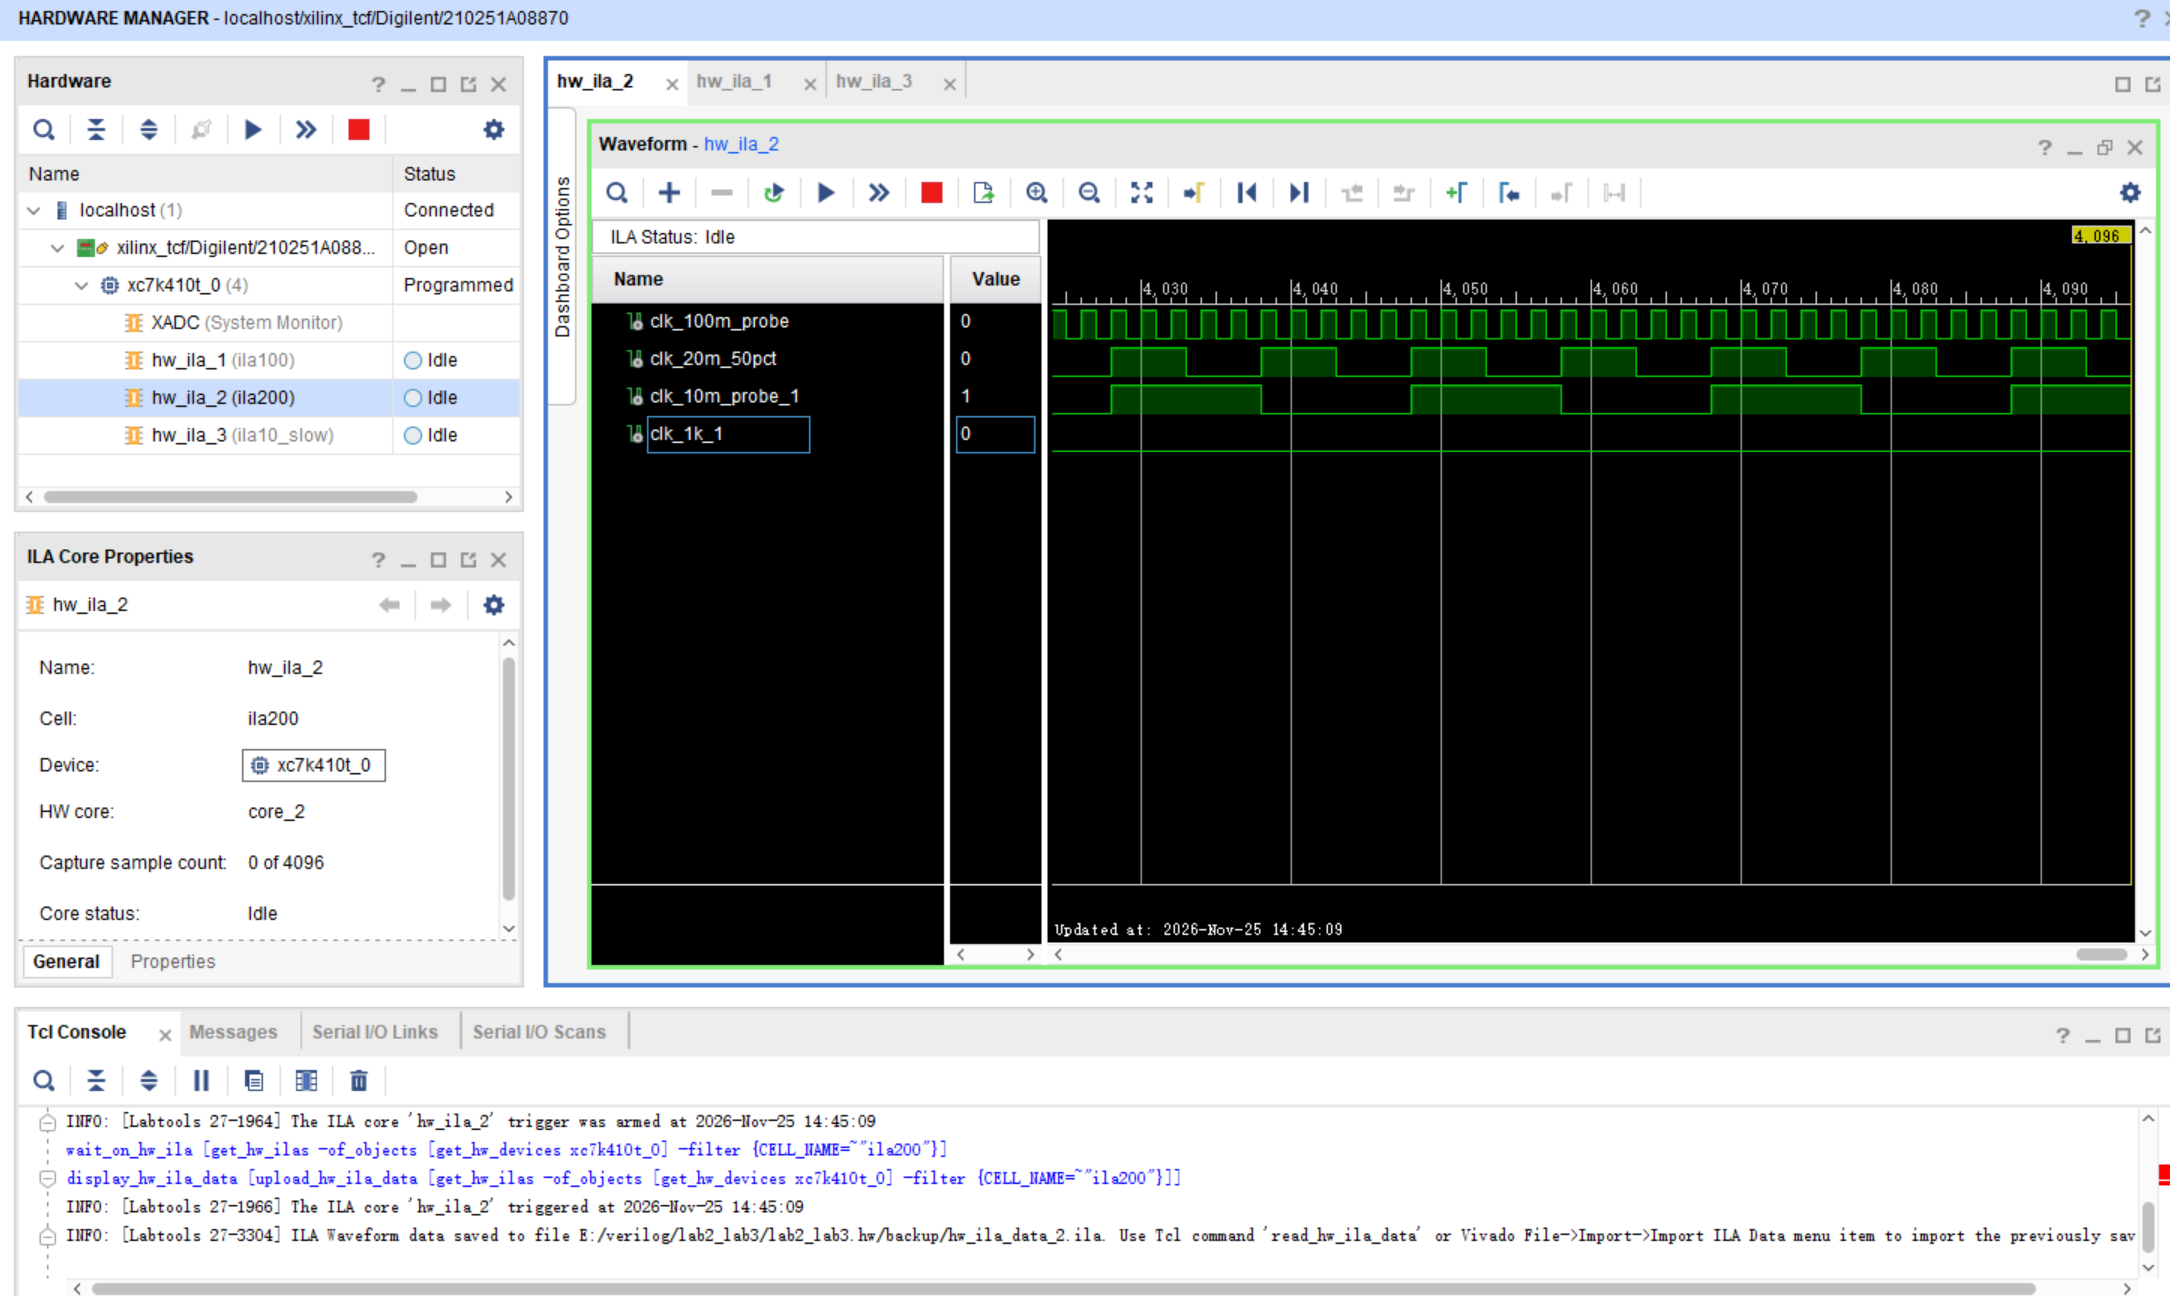
\includegraphics[width=\linewidth]{sections/ex2/picture/board_200mhz.png}
    \caption{200\,MHz ILA 同步采集的四路时钟，横轴每个采样间隔为 5\,ns}
    \label{fig:ex2-fast-clocks}
\end{figure}

图~\ref{fig:ex2-fast-clocks} 中最下方的 1\,kHz 探针在当前视图内持续为低电平。即使展开全部 4096 点，记录也仅覆盖 $20.48\,\mu\mathrm{s}$，而 1\,kHz 的一个周期为 1\,ms。图~\ref{fig:ex2-1khz-period} 改用 10\,MHz 采样，记录窗口延长到 1.6384\,ms。图中相邻两个上升沿相隔约 10\,000 个采样间隔，高电平约占其中一半。

\begin{figure}[H]
    \centering
    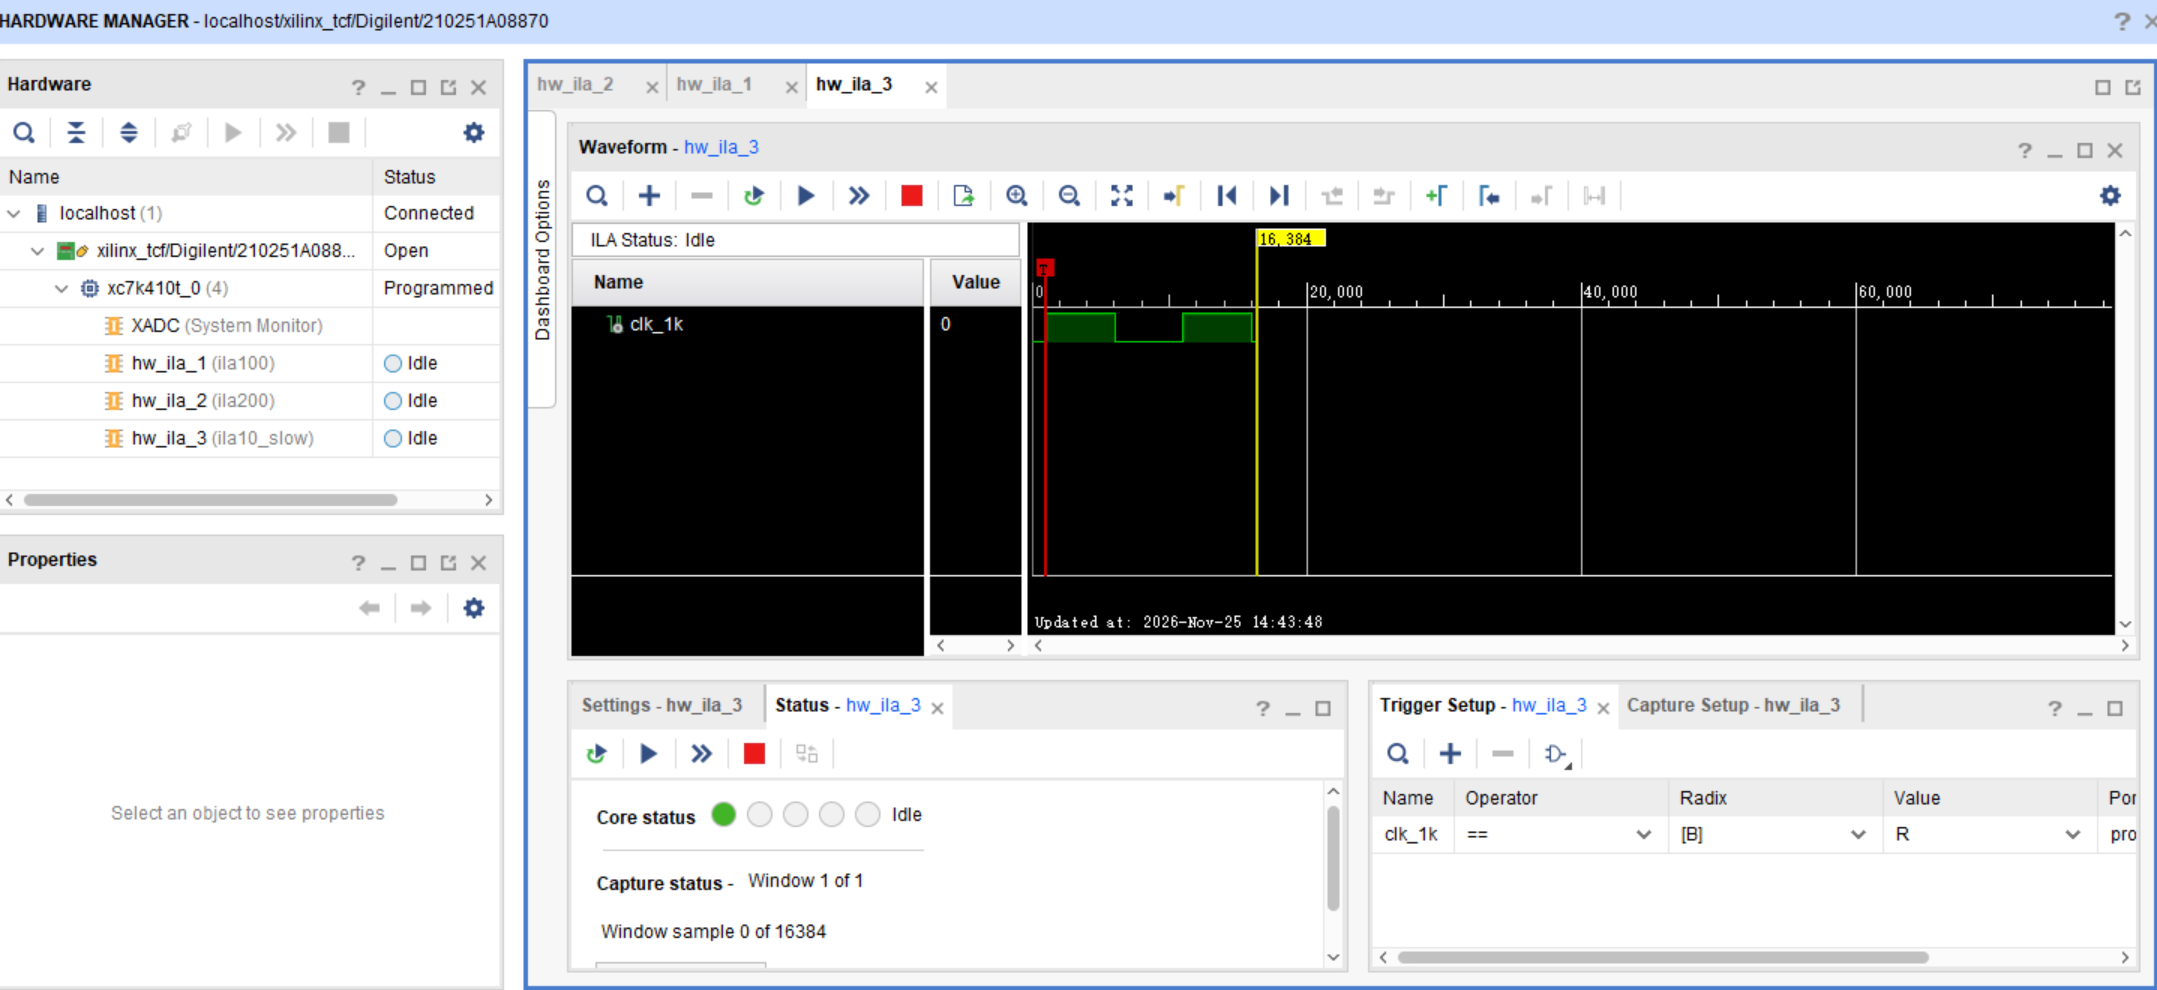
\includegraphics[width=\linewidth]{sections/ex2/picture/board_1khz.png}
    \caption{10\,MHz ILA 采集的 1\,kHz 波形。有效记录共 16\,384 点，每点间隔 100\,ns}
    \label{fig:ex2-1khz-period}
\end{figure}

\begin{table}[H]
    \centering
    \caption{根据板上波形估算的时钟周期和占空比}
    \label{tab:ex2-ila-clocks}
    \small
    \begin{tabular}{lrrrr}
        \toprule
        被测时钟 & 采样频率 & 每周期样点数 & 周期估计 & 占空比估计 \\
        \midrule
        100\,MHz & 200\,MHz & 2 & 10\,ns & 约 50\% \\
         20\,MHz & 200\,MHz & 10 & 50\,ns & 约 50\% \\
         10\,MHz & 200\,MHz & 20 & 100\,ns & 约 50\% \\
          1\,kHz & 10\,MHz & 约 10\,000 & 约 1\,ms & 约 50\% \\
        \bottomrule
    \end{tabular}
\end{table}

表~\ref{tab:ex2-ila-clocks} 中四路波形的周期均与设计值一致。100\,MHz 信号每周期只有一高一低两个样点，能辨认电平交替，但 5\,ns 的采样间隔限制了对其高电平宽度的测量精度。
